\documentclass[11pt,a4paper]{article}

\usepackage[T1]{fontenc}
\usepackage[utf8]{inputenc}
\usepackage{lmodern}
\usepackage{microtype}
\usepackage[margin=2.3cm]{geometry}
\usepackage{amsmath,amssymb,amsthm}
\usepackage{booktabs,tabularx,array}
\usepackage{graphicx}
\usepackage{float}
\usepackage[font=small,labelfont=bf]{caption}
\usepackage{xcolor}
\usepackage{listings}
\usepackage{algorithm}
\usepackage{algpseudocode}
\usepackage{enumitem}
\usepackage{fancyhdr}
\usepackage[colorlinks=true,linkcolor=blue!50!black,citecolor=blue!50!black,urlcolor=blue!50!black]{hyperref}

\graphicspath{{../figures/}}
% Generated from the project dataset by make_report_tables.py -- do not edit by hand.
\newcommand{\SitesTable}{
\begin{table}[H]\centering\small
\caption{The ten vertices: real coordinates (OpenStreetMap), assumed damage class, and distance to the nearest road intersection.}\label{tab:sites}
\setlength{\tabcolsep}{4pt}
\begin{tabular}{clllrrr}
\toprule
\# & Site & Category & Latitude & Longitude & $d_i$ (min) & Snap (m) \\
\midrule
0 & Cagayan de Oro City Hall & Depot & 8.47695 & 124.64117 & 0 & 89 \\
1 & Northern Mindanao Medical Center & Hospital & 8.48539 & 124.64964 & 0 & 81 \\
2 & J. R. Borja Memorial City Hospital & Hospital & 8.48171 & 124.62809 & 5 & 82 \\
3 & Capitol University Hospital & Hospital & 8.47905 & 124.67268 & 0 & 87 \\
4 & Maria Reyna--Xavier University Hospital & Hospital & 8.47631 & 124.65520 & 0 & 37 \\
5 & Balulang Elementary School & Evacuation & 8.44344 & 124.63451 & 20 & 77 \\
6 & Macasandig Multipurpose Covered Court & Evacuation & 8.46535 & 124.64478 & 20 & 37 \\
7 & Carmen National High School & Evacuation & 8.46950 & 124.63234 & 5 & 45 \\
8 & West City Central School & Evacuation & 8.47350 & 124.63686 & 5 & 59 \\
9 & Philippine Red Cross -- CDO Chapter & Response hub & 8.48477 & 124.64926 & 0 & 127 \\
\bottomrule
\end{tabular}
\end{table}}
\newcommand{\TravelMatrix}{\begin{table}[H]\centering\small
\caption{Actual travel-time matrix $t(i,j)$ in minutes: fastest path on the OpenStreetMap drive network (row = from, column = to).}\label{tab:travel}
\begin{tabular}{c|rrrrrrrrrr}
\toprule
from $\backslash$ to & \textbf{0} & \textbf{1} & \textbf{2} & \textbf{3} & \textbf{4} & \textbf{5} & \textbf{6} & \textbf{7} & \textbf{8} & \textbf{9} \\
\midrule
\textbf{0} & -- & 2.5 & 3.4 & 6.4 & 3.3 & 9.7 & 3.3 & 3.3 & 1.6 & 2.6 \\
\textbf{1} & 2.8 & -- & 5.5 & 3.9 & 3.3 & 12.1 & 5.2 & 6.0 & 4.4 & 0.7 \\
\textbf{2} & 3.4 & 5.2 & -- & 9.1 & 6.4 & 11.2 & 6.1 & 4.7 & 3.4 & 5.6 \\
\textbf{3} & 6.4 & 4.0 & 9.1 & -- & 5.0 & 15.7 & 8.8 & 9.6 & 8.0 & 4.3 \\
\textbf{4} & 3.3 & 3.4 & 6.5 & 5.0 & -- & 12.5 & 4.7 & 6.5 & 4.9 & 3.0 \\
\textbf{5} & 9.7 & 11.8 & 11.2 & 15.7 & 12.1 & -- & 8.5 & 7.2 & 9.1 & 11.9 \\
\textbf{6} & 3.5 & 5.1 & 6.5 & 8.9 & 4.5 & 8.5 & -- & 5.3 & 4.2 & 4.9 \\
\textbf{7} & 3.3 & 5.6 & 4.7 & 9.6 & 6.5 & 7.2 & 4.7 & -- & 2.6 & 5.8 \\
\textbf{8} & 1.6 & 4.0 & 3.4 & 7.9 & 4.9 & 9.1 & 3.7 & 2.7 & -- & 4.1 \\
\textbf{9} & 2.6 & 0.8 & 5.6 & 4.3 & 3.0 & 11.9 & 4.8 & 5.8 & 4.1 & -- \\
\bottomrule
\end{tabular}
\end{table}
}
\newcommand{\DistanceMatrix}{\begin{table}[H]\centering\small
\caption{Road distance in kilometres along the same fastest paths.}\label{tab:distance}
\begin{tabular}{c|rrrrrrrrrr}
\toprule
from $\backslash$ to & \textbf{0} & \textbf{1} & \textbf{2} & \textbf{3} & \textbf{4} & \textbf{5} & \textbf{6} & \textbf{7} & \textbf{8} & \textbf{9} \\
\midrule
\textbf{0} & -- & 1.59 & 1.74 & 4.22 & 1.76 & 5.00 & 1.65 & 1.86 & 0.89 & 1.55 \\
\textbf{1} & 1.82 & -- & 3.35 & 2.63 & 1.75 & 6.82 & 3.00 & 3.70 & 2.73 & 0.37 \\
\textbf{2} & 1.75 & 3.10 & -- & 5.73 & 3.17 & 5.40 & 3.04 & 2.25 & 1.62 & 2.94 \\
\textbf{3} & 4.22 & 2.67 & 5.74 & -- & 2.84 & 9.21 & 5.40 & 6.10 & 5.13 & 2.79 \\
\textbf{4} & 1.76 & 1.82 & 3.18 & 2.84 & -- & 6.58 & 2.29 & 3.64 & 2.67 & 1.48 \\
\textbf{5} & 5.00 & 6.57 & 5.39 & 9.20 & 6.40 & -- & 4.56 & 3.39 & 4.43 & 6.53 \\
\textbf{6} & 1.64 & 2.79 & 3.29 & 4.98 & 2.15 & 4.03 & -- & 2.53 & 1.95 & 2.37 \\
\textbf{7} & 1.86 & 3.45 & 2.25 & 6.08 & 3.62 & 3.39 & 2.32 & -- & 1.28 & 3.41 \\
\textbf{8} & 0.90 & 2.50 & 1.62 & 5.13 & 2.67 & 4.45 & 1.76 & 1.30 & -- & 2.46 \\
\textbf{9} & 1.54 & 0.43 & 2.94 & 2.78 & 1.48 & 6.53 & 2.37 & 3.42 & 2.45 & -- \\
\bottomrule
\end{tabular}
\end{table}
}
\newcommand{\ClearingMatrix}{\begin{table}[H]\centering\small
\caption{Assumed clearing-time matrix $c(i,j)=\max(d_i,d_j)$ in minutes.}\label{tab:clearing}
\begin{tabular}{c|rrrrrrrrrr}
\toprule
from $\backslash$ to & \textbf{0} & \textbf{1} & \textbf{2} & \textbf{3} & \textbf{4} & \textbf{5} & \textbf{6} & \textbf{7} & \textbf{8} & \textbf{9} \\
\midrule
\textbf{0} & -- & 0 & 5 & 0 & 0 & 20 & 20 & 5 & 5 & 0 \\
\textbf{1} & 0 & -- & 5 & 0 & 0 & 20 & 20 & 5 & 5 & 0 \\
\textbf{2} & 5 & 5 & -- & 5 & 5 & 20 & 20 & 5 & 5 & 5 \\
\textbf{3} & 0 & 0 & 5 & -- & 0 & 20 & 20 & 5 & 5 & 0 \\
\textbf{4} & 0 & 0 & 5 & 0 & -- & 20 & 20 & 5 & 5 & 0 \\
\textbf{5} & 20 & 20 & 20 & 20 & 20 & -- & 20 & 20 & 20 & 20 \\
\textbf{6} & 20 & 20 & 20 & 20 & 20 & 20 & -- & 20 & 20 & 20 \\
\textbf{7} & 5 & 5 & 5 & 5 & 5 & 20 & 20 & -- & 5 & 5 \\
\textbf{8} & 5 & 5 & 5 & 5 & 5 & 20 & 20 & 5 & -- & 5 \\
\textbf{9} & 0 & 0 & 5 & 0 & 0 & 20 & 20 & 5 & 5 & -- \\
\bottomrule
\end{tabular}
\end{table}
}
\newcommand{\WeightMatrix}{\begin{table}[H]\centering\small
\caption{Combined weight matrix $w(i,j)=t(i,j)+c(i,j)$ in minutes, used by Algorithm 2.7.}\label{tab:weights}
\begin{tabular}{c|rrrrrrrrrr}
\toprule
from $\backslash$ to & \textbf{0} & \textbf{1} & \textbf{2} & \textbf{3} & \textbf{4} & \textbf{5} & \textbf{6} & \textbf{7} & \textbf{8} & \textbf{9} \\
\midrule
\textbf{0} & -- & 2.5 & 8.4 & 6.4 & 3.3 & 29.7 & 23.3 & 8.3 & 6.6 & 2.6 \\
\textbf{1} & 2.8 & -- & 10.5 & 3.9 & 3.3 & 32.1 & 25.2 & 11.0 & 9.4 & 0.7 \\
\textbf{2} & 8.4 & 10.2 & -- & 14.1 & 11.4 & 31.2 & 26.1 & 9.7 & 8.4 & 10.6 \\
\textbf{3} & 6.4 & 4.0 & 14.1 & -- & 5.0 & 35.7 & 28.8 & 14.6 & 13.0 & 4.3 \\
\textbf{4} & 3.3 & 3.4 & 11.5 & 5.0 & -- & 32.5 & 24.7 & 11.5 & 9.9 & 3.0 \\
\textbf{5} & 29.7 & 31.8 & 31.2 & 35.7 & 32.1 & -- & 28.5 & 27.2 & 29.1 & 31.9 \\
\textbf{6} & 23.5 & 25.1 & 26.5 & 28.9 & 24.5 & 28.5 & -- & 25.3 & 24.2 & 24.9 \\
\textbf{7} & 8.3 & 10.6 & 9.7 & 14.6 & 11.5 & 27.2 & 24.7 & -- & 7.6 & 10.8 \\
\textbf{8} & 6.6 & 9.0 & 8.4 & 12.9 & 9.9 & 29.1 & 23.7 & 7.7 & -- & 9.1 \\
\textbf{9} & 2.6 & 0.8 & 10.6 & 4.3 & 3.0 & 31.9 & 24.8 & 10.8 & 9.1 & -- \\
\bottomrule
\end{tabular}
\end{table}
}
\newcommand{\StepTable}{
\begin{table}[H]\centering\small
\caption{Trace of Algorithm 2.7 from the depot. At each step the three nearest unvisited sites are listed as \emph{site: $w$}; the smallest is chosen.}\label{tab:steps}
\begin{tabular}{clp{5.2cm}rrrr}
\toprule
Step & Leg & Nearest unvisited candidates & $t$ & $c$ & $w$ & Running total \\
\midrule
1 & 0 $\to$ 1 & 1: 2.5, 9: 2.6, 4: 3.3 & 2.5 & 0 & \textbf{2.5} & 2.5 \\
2 & 1 $\to$ 9 & 9: 0.7, 4: 3.3, 3: 3.9 & 0.7 & 0 & \textbf{0.7} & 3.2 \\
3 & 9 $\to$ 4 & 4: 3.0, 3: 4.3, 8: 9.1 & 3.0 & 0 & \textbf{3.0} & 6.2 \\
4 & 4 $\to$ 3 & 3: 5.0, 8: 9.9, 2: 11.5 & 5.0 & 0 & \textbf{5.0} & 11.2 \\
5 & 3 $\to$ 8 & 8: 13.0, 2: 14.1, 7: 14.6 & 8.0 & 5 & \textbf{13.0} & 24.2 \\
6 & 8 $\to$ 7 & 7: 7.7, 2: 8.4, 6: 23.7 & 2.7 & 5 & \textbf{7.7} & 31.9 \\
7 & 7 $\to$ 2 & 2: 9.7, 6: 24.7, 5: 27.2 & 4.7 & 5 & \textbf{9.7} & 41.6 \\
8 & 2 $\to$ 6 & 6: 26.1, 5: 31.2 & 6.1 & 20 & \textbf{26.1} & 67.7 \\
9 & 6 $\to$ 5 & 5: 28.5 & 8.5 & 20 & \textbf{28.5} & 96.2 \\
10 & 5 $\to$ 0 & return to depot & 9.7 & 20 & \textbf{29.7} & 125.9 \\
\bottomrule
\end{tabular}
\end{table}}
\newcommand{\SensitivityTable}{
\begin{table}[H]\centering\small
\caption{Greedy result when started from each site. Every closed tour is a cycle, so its total is also a valid depot round trip.}\label{tab:sensitivity}
\begin{tabular}{cllr}
\toprule
Start & Site & Greedy tour & Total (min) \\
\midrule
0 & City Hall & 0 $\to$ 1 $\to$ 9 $\to$ 4 $\to$ 3 $\to$ 8 $\to$ 7 $\to$ 2 $\to$ 6 $\to$ 5 $\to$ 0 & 125.9 \\
1 & NMMC & 1 $\to$ 9 $\to$ 0 $\to$ 4 $\to$ 3 $\to$ 8 $\to$ 7 $\to$ 2 $\to$ 6 $\to$ 5 $\to$ 1 & 128.4 \\
2 & J.R. Borja & 2 $\to$ 0 $\to$ 1 $\to$ 9 $\to$ 4 $\to$ 3 $\to$ 8 $\to$ 7 $\to$ 6 $\to$ 5 $\to$ 2 & 124.7 \\
3 & Capitol Univ. & 3 $\to$ 1 $\to$ 9 $\to$ 0 $\to$ 4 $\to$ 8 $\to$ 7 $\to$ 2 $\to$ 6 $\to$ 5 $\to$ 3 & 128.2 \\
4 & Maria Reyna & 4 $\to$ 9 $\to$ 1 $\to$ 0 $\to$ 3 $\to$ 8 $\to$ 7 $\to$ 2 $\to$ 6 $\to$ 5 $\to$ 4 & 130.1 \\
5 & Balulang ES & 5 $\to$ 7 $\to$ 8 $\to$ 0 $\to$ 1 $\to$ 9 $\to$ 4 $\to$ 3 $\to$ 2 $\to$ 6 $\to$ 5 & 121.3 \\
6 & Macasandig CC & 6 $\to$ 0 $\to$ 1 $\to$ 9 $\to$ 4 $\to$ 3 $\to$ 8 $\to$ 7 $\to$ 2 $\to$ 5 $\to$ 6 & 124.8 \\
7 & Carmen NHS & 7 $\to$ 8 $\to$ 0 $\to$ 1 $\to$ 9 $\to$ 4 $\to$ 3 $\to$ 2 $\to$ 6 $\to$ 5 $\to$ 7 & 121.3 \\
8 & West City CS & 8 $\to$ 0 $\to$ 1 $\to$ 9 $\to$ 4 $\to$ 3 $\to$ 2 $\to$ 7 $\to$ 6 $\to$ 5 $\to$ 8 & 123.9 \\
9 & Red Cross & 9 $\to$ 1 $\to$ 0 $\to$ 4 $\to$ 3 $\to$ 8 $\to$ 7 $\to$ 2 $\to$ 6 $\to$ 5 $\to$ 9 & 128.8 \\
\bottomrule
\end{tabular}
\end{table}}
\newcommand{\OptimalTable}{
\begin{table}[H]\centering\small
\caption{Exact optimal tour (Held--Karp dynamic programming), leg by leg.}\label{tab:optimal}
\begin{tabular}{cllrrr}
\toprule
Leg & Sites & $t$ & $c$ & $w$ & Running total \\
\midrule
0 $\to$ 2 & City Hall $\to$ J.R. Borja & 3.4 & 5 & 8.4 & 8.4 \\
2 $\to$ 8 & J.R. Borja $\to$ West City CS & 3.4 & 5 & 8.4 & 16.8 \\
8 $\to$ 7 & West City CS $\to$ Carmen NHS & 2.7 & 5 & 7.7 & 24.5 \\
7 $\to$ 5 & Carmen NHS $\to$ Balulang ES & 7.2 & 20 & 27.2 & 51.7 \\
5 $\to$ 6 & Balulang ES $\to$ Macasandig CC & 8.5 & 20 & 28.5 & 80.2 \\
6 $\to$ 4 & Macasandig CC $\to$ Maria Reyna & 4.5 & 20 & 24.5 & 104.7 \\
4 $\to$ 3 & Maria Reyna $\to$ Capitol Univ. & 5.0 & 0 & 5.0 & 109.7 \\
3 $\to$ 1 & Capitol Univ. $\to$ NMMC & 4.0 & 0 & 4.0 & 113.7 \\
1 $\to$ 9 & NMMC $\to$ Red Cross & 0.7 & 0 & 0.7 & 114.4 \\
9 $\to$ 0 & Red Cross $\to$ City Hall & 2.6 & 0 & 2.6 & 117.0 \\
\bottomrule
\end{tabular}
\end{table}}
\newcommand{\GreedyTotal}{125.9}
\newcommand{\GreedyTravel}{50.9}
\newcommand{\GreedyClear}{75}
\newcommand{\GreedyKm}{27.03}
\newcommand{\OptTotal}{117.0}
\newcommand{\OptTravel}{42.0}
\newcommand{\OptClear}{75}
\newcommand{\OptKm}{22.18}
\newcommand{\GapPct}{7.6}
\newcommand{\GapMin}{8.9}


\definecolor{codebg}{RGB}{247,245,240}
\definecolor{codekw}{RGB}{200,70,10}
\definecolor{codecm}{RGB}{110,115,125}
\definecolor{codestr}{RGB}{30,110,60}
\lstdefinestyle{py}{
  language=Python, basicstyle=\ttfamily\scriptsize, backgroundcolor=\color{codebg},
  keywordstyle=\color{codekw}\bfseries, commentstyle=\color{codecm}\itshape, stringstyle=\color{codestr},
  numbers=left, numberstyle=\tiny\color{codecm}, numbersep=6pt, frame=single, rulecolor=\color{codebg},
  breaklines=true, breakatwhitespace=true, showstringspaces=false, columns=fullflexible, keepspaces=true,
  tabsize=4, xleftmargin=1.5em, framexleftmargin=1.5em
}
\lstdefinestyle{out}{basicstyle=\ttfamily\scriptsize, backgroundcolor=\color{codebg}, frame=single,
  rulecolor=\color{codebg}, columns=fullflexible, keepspaces=true, breaklines=true}

\newtheorem{theorem}{Theorem}
\renewcommand{\theequation}{\arabic{equation}}

\pagestyle{fancy}
\fancyhf{}
\fancyhead[L]{\small Greedy TSP for Post-Disaster Response}
\fancyhead[R]{\small Cagayan de Oro City}
\fancyfoot[C]{\small\thepage}
\renewcommand{\headrulewidth}{0.4pt}

\title{\textbf{Greedy Routing for Post-Disaster Emergency Response in Cagayan de Oro City}\\[0.6em]
\large A Traveling Salesperson Problem solved with Algorithm 2.7 (Greedy / Nearest-Neighbor)\\ on the real OpenStreetMap road network}
\author{Jhey Gulde\\[0.2em]
\small University of Science and Technology of Southern Philippines\\
\small Performance Innovative Task -- Algorithm Discussion and Real-Life Application of the TSP}
\date{October 2026}

\begin{document}
\maketitle
\thispagestyle{empty}

\begin{abstract}
\noindent After a typhoon, an emergency response crew in Cagayan de Oro City must leave a central depot, reach ten critical sites (hospitals, evacuation centers and a response hub) exactly once, and return, in the shortest possible time. We model this as a directed, weighted Traveling Salesperson Problem (TSP). Site coordinates come from OpenStreetMap; travel times are fastest paths on the city's real drivable road network (5,835 intersections), and a road-clearing penalty models flood damage. We apply Algorithm 2.7 of Luna-Garcia, Candano and Caga-anan (2024), the Greedy (Nearest-Neighbor) approach, and implement it in Python. Starting from City Hall, the greedy tour takes \textbf{\GreedyTotal{} minutes} and is verified to visit every site exactly once. An exact Held--Karp dynamic program, confirmed by brute force over all $9! = 362{,}880$ tours, gives an optimum of \textbf{\OptTotal{} minutes}: the greedy tour is \GapPct\% longer. Because both tours spend the same \GreedyClear{} minutes clearing roads, the whole gap comes from driving. The result illustrates the algorithm's main trade-off: a fast, valid, easily explained route that is approximate rather than optimal.
\end{abstract}

\tableofcontents
\newpage

%=====================================================================
\section{Introduction}
%=====================================================================
The Traveling Salesperson Problem (TSP) asks for a route that visits each of a given set of locations exactly once and returns to the starting location while minimizing the total distance, travel time or cost. It is one of the most studied problems in combinatorial optimization and is NP-hard: the number of possible tours grows factorially with the number of locations, so exact methods quickly become impractical \cite{luna2024}.

This report documents a complete application of the TSP to a real situation in Cagayan de Oro City. It follows the structure of the Performance Innovative Task:
\begin{enumerate}[noitemsep]
  \item a discussion of the assigned algorithm, Algorithm 2.7 (Greedy), including its procedure, complexity, advantages, limitations and optimality (Section~\ref{sec:algorithm});
  \item the real-life problem, its locations, assumptions, constraints and objective (Section~\ref{sec:problem});
  \item the weighted graph model and the data behind it, with actual and assumed data clearly separated (Section~\ref{sec:model});
  \item the application of the algorithm with all key calculations (Section~\ref{sec:apply});
  \item the Python implementation (Section~\ref{sec:python});
  \item the results, their verification and an optimality check (Section~\ref{sec:results}); and
  \item conclusions, limitations and possible improvements (Section~\ref{sec:conclusion}).
\end{enumerate}

\paragraph{Summary of results.} The greedy round trip from City Hall is $0 \to 1 \to 9 \to 4 \to 3 \to 8 \to 7 \to 2 \to 6 \to 5 \to 0$ with a total of \GreedyTotal{} minutes (\GreedyTravel{} minutes driving, \GreedyClear{} minutes clearing, \GreedyKm{} km). The exact optimum is \OptTotal{} minutes, so the greedy solution is \GapMin{} minutes (\GapPct\%) longer.

%=====================================================================
\section{The assigned algorithm: Algorithm 2.7 (Greedy)}\label{sec:algorithm}
%=====================================================================
\subsection{Idea}
A greedy algorithm builds a solution step by step and, at every step, takes the choice that looks best \emph{right now}, without considering its long-term consequences \cite{luna2024}. For the TSP this choice is simple: from the current location, travel to the \emph{nearest location that has not been visited yet}. For this reason the method is also called the Nearest-Neighbor heuristic. It never backtracks or revises an earlier choice.

\subsection{Procedure}
Algorithm~\ref{alg:paper} reproduces the pseudocode of Algorithm 2.7 from the paper. Algorithm~\ref{alg:formal} states the same procedure precisely, in the form that our Python code implements, for a weight matrix $W$ and a starting vertex $s$.

\begin{algorithm}[H]
\caption{Algorithm 2.7 -- Greedy Algorithm Approach for TSP (Luna-Garcia et al., 2024, p.~89)}\label{alg:paper}
\begin{algorithmic}[1]
\State \textbf{Input:} cities and pairwise distances
\State Begin at an arbitrary city
\While{not all cities have been visited}
  \State Find the nearest unvisited city (based on the distance) and travel to it
  \State Mark the city as visited
\EndWhile
\State Return to the starting city to complete the tour
\State \textbf{Output:} complete tour with the total distance
\end{algorithmic}
\end{algorithm}

\begin{algorithm}[H]
\caption{Greedy TSP, formal version (as implemented in \texttt{greedy\_tsp})}\label{alg:formal}
\begin{algorithmic}[1]
\Require weight matrix $W \in \mathbb{R}^{n \times n}$, start vertex $s$
\State $\mathit{tour} \gets [s]$;\quad $\mathit{visited} \gets \{s\}$;\quad $\mathit{total} \gets 0$;\quad $u \gets s$
\While{$|\mathit{tour}| < n$}
  \State $v \gets \arg\min_{j \notin \mathit{visited}} W[u][j]$ \Comment{nearest unvisited vertex}
  \State append $v$ to $\mathit{tour}$;\quad $\mathit{visited} \gets \mathit{visited} \cup \{v\}$
  \State $\mathit{total} \gets \mathit{total} + W[u][v]$;\quad $u \gets v$
\EndWhile
\State $\mathit{total} \gets \mathit{total} + W[u][s]$;\quad append $s$ to $\mathit{tour}$ \Comment{close the loop}
\State \Return $\mathit{tour}, \mathit{total}$
\end{algorithmic}
\end{algorithm}

Step by step:
\begin{enumerate}[noitemsep]
  \item \textbf{Initialize.} Put the starting vertex in the tour and mark it visited.
  \item \textbf{Look around.} From the current vertex $u$, read the weights $W[u][j]$ to every unvisited vertex $j$.
  \item \textbf{Choose greedily.} Pick the unvisited vertex $v$ with the smallest weight. Ties are broken by the lowest index.
  \item \textbf{Move.} Add $v$ to the tour, mark it visited, add $W[u][v]$ to the total and make $v$ the current vertex.
  \item \textbf{Repeat} steps 2--4 until every vertex is in the tour.
  \item \textbf{Close the tour} by returning from the last vertex to the start and adding that weight.
\end{enumerate}
Because every vertex is added exactly once and the tour ends at the start, the output is always a valid closed tour (a Hamiltonian cycle).

\subsection{Time complexity}
\begin{theorem}[Theorem 2.7 in \cite{luna2024}]
For $n$ cities, the greedy approach for the TSP runs in $O(n^2)$ time.
\end{theorem}
\begin{proof}
Choosing the start and initializing the arrays costs $O(n)$. The loop runs $n-1$ times. In each iteration, finding the nearest unvisited vertex scans at most $n$ entries of one row of $W$, which is $O(n)$; marking the vertex and updating the total are $O(1)$. The loop therefore costs $(n-1)\cdot O(n) = O(n^2)$. Closing the tour is $O(1)$. The total is $T(n) = O(n) + O(n^2) + O(1) = O(n^2)$.
\end{proof}
\noindent For our $n = 10$ sites this is at most $9 \times 10 = 90$ comparisons. The algorithm needs $O(n^2)$ memory for the weight matrix and $O(n)$ for the tour. For comparison, the exact methods in the same paper cost $O(n^2 2^n)$ (dynamic programming) and $O(n!)$ (brute force).

\subsection{Advantages}
\begin{itemize}[noitemsep]
  \item \textbf{Fast and scalable.} $O(n^2)$ time handles thousands of locations; the paper's experiments run it on up to 256 cities.
  \item \textbf{Simple.} It needs only a distance matrix and a visited list, and it is easy to explain to a field team.
  \item \textbf{Always valid.} It always returns a closed tour that visits every location exactly once.
  \item \textbf{Deterministic.} For a fixed start (and tie-breaking rule) it always gives the same tour, so results are reproducible.
  \item \textbf{A good starting point.} Its tour is a common initial solution for improvement methods such as 2-opt \cite{croes1958}.
\end{itemize}

\subsection{Limitations}
\begin{itemize}[noitemsep]
  \item \textbf{Myopic.} Taking the shortest edge now can force very long edges later, especially the last legs and the return to the start.
  \item \textbf{Sensitive to the starting vertex.} Different starts give different tours and totals (Table~\ref{tab:sensitivity}).
  \item \textbf{No quality guarantee in general.} For metric instances its tour can be up to $\tfrac12(\lceil \log_2 n\rceil + 1)$ times the optimum \cite{rosenkrantz1977}, and without the triangle inequality it can be arbitrarily bad.
  \item \textbf{No backtracking.} Unlike simulated annealing, genetic algorithms or particle swarm optimization \cite{luna2024}, it cannot undo a poor early choice.
\end{itemize}

\subsection{Optimality}
\textbf{The greedy approach does not guarantee an optimal solution; it produces an approximate (heuristic) solution.} Each step is locally optimal, but the combined tour is generally not globally optimal. In this project we therefore claim optimality only for the exact Held--Karp dynamic program used as a check in Section~\ref{sec:optimal}, never for the greedy tour.

%=====================================================================
\section{Problem and objective}\label{sec:problem}
%=====================================================================
\subsection{Real-life situation}
Cagayan de Oro City lies on the Cagayan River and has suffered severe river flooding, most notably during Tropical Storm Sendong (Washi) in December 2011. We consider a similar scenario: a typhoon has flooded and blocked roads across the city. A single emergency response crew leaves a central depot to deliver supplies and assess damage at every critical site, and must then return to the depot. Every minute on the road delays help at the remaining sites, so the order of visits matters.

\subsection{Locations}
The starting location (depot) is Cagayan de Oro City Hall. The nine required locations are four hospitals, four evacuation sites and one emergency response hub (Table~\ref{tab:sites}). All coordinates were looked up on OpenStreetMap. City Hall is used as the depot because the only disaster-office entry in OpenStreetMap is in the provincial Capitol area and may be the provincial office. Schools are used as evacuation sites because OpenStreetMap does not tag evacuation centers explicitly.

\SitesTable

\subsection{Assumptions}
\begin{enumerate}[noitemsep]
  \item \textbf{Driving speeds} depend on road class (Table~\ref{tab:speeds}): 20--40 km/h, typical of urban traffic. OpenStreetMap \texttt{maxspeed} tags are used where present.
  \item \textbf{Road clearing} adds a delay at each site's access roads according to an assumed damage class: 0 (clear), 5 (minor debris) or 20 minutes (major obstruction).
  \item \textbf{Riverside sites are hardest hit.} Balulang and Macasandig, along the Cagayan River, are assigned major obstruction; J. R. Borja, Carmen and West City, minor debris; the others are clear.
  \item \textbf{Schools serve as evacuation centers.}
  \item \textbf{Service time} at each site is not modeled, and the short walk from a building to the nearest road intersection (at most 127 m) is ignored.
  \item \textbf{The network is static}: travel and clearing times do not change during the trip.
\end{enumerate}

\subsection{Constraints}
\begin{enumerate}[noitemsep]
  \item The tour starts and ends at the depot (vertex 0).
  \item Each of the other nine sites is visited exactly once.
  \item One crew with one vehicle travels on drivable roads only.
  \item Road direction is respected: one-way streets may only be driven in their allowed direction.
  \item There are no time windows, capacity limits or site priorities.
\end{enumerate}

\subsection{Objective}
Minimize the \textbf{total round-trip time in minutes}. For a tour $\pi = (\pi_0, \pi_1, \dots, \pi_{n-1}, \pi_n)$ with $\pi_0 = \pi_n = 0$ that visits every site once,
\begin{equation}
  \min_{\pi} \; T(\pi) = \sum_{k=0}^{n-1} w(\pi_k, \pi_{k+1}), \qquad w(i,j) = t(i,j) + c(i,j),
\end{equation}
where $t(i,j)$ is the driving time and $c(i,j)$ is the road-clearing time from site $i$ to site $j$.

%=====================================================================
\section{Methodology and graph model}\label{sec:model}
%=====================================================================
\subsection{Weighted graph}
The problem is modeled as a complete weighted directed graph $G = (V, E, w)$.
\begin{itemize}[noitemsep]
  \item \textbf{Vertices} $V = \{0, 1, \dots, 9\}$: the ten sites of Table~\ref{tab:sites}; vertex 0 is the depot.
  \item \textbf{Edges} $E = \{(i,j) : i \neq j\}$: the fastest road route from site $i$ to site $j$ on the real network, giving $10 \times 9 = 90$ directed edges.
  \item \textbf{Direction.} Travel is \emph{directed}, because one-way streets make the fastest route from $i$ to $j$ differ from the route from $j$ to $i$. In our data, 20 of the 45 site pairs differ by direction, by at most 0.6 minutes.
  \item \textbf{Weights} $w(i,j) = t(i,j) + c(i,j)$, in minutes.
\end{itemize}
Figure~\ref{fig:graph} shows the labeled graph with vertices at their real relative positions.

\begin{figure}[H]
  \centering
  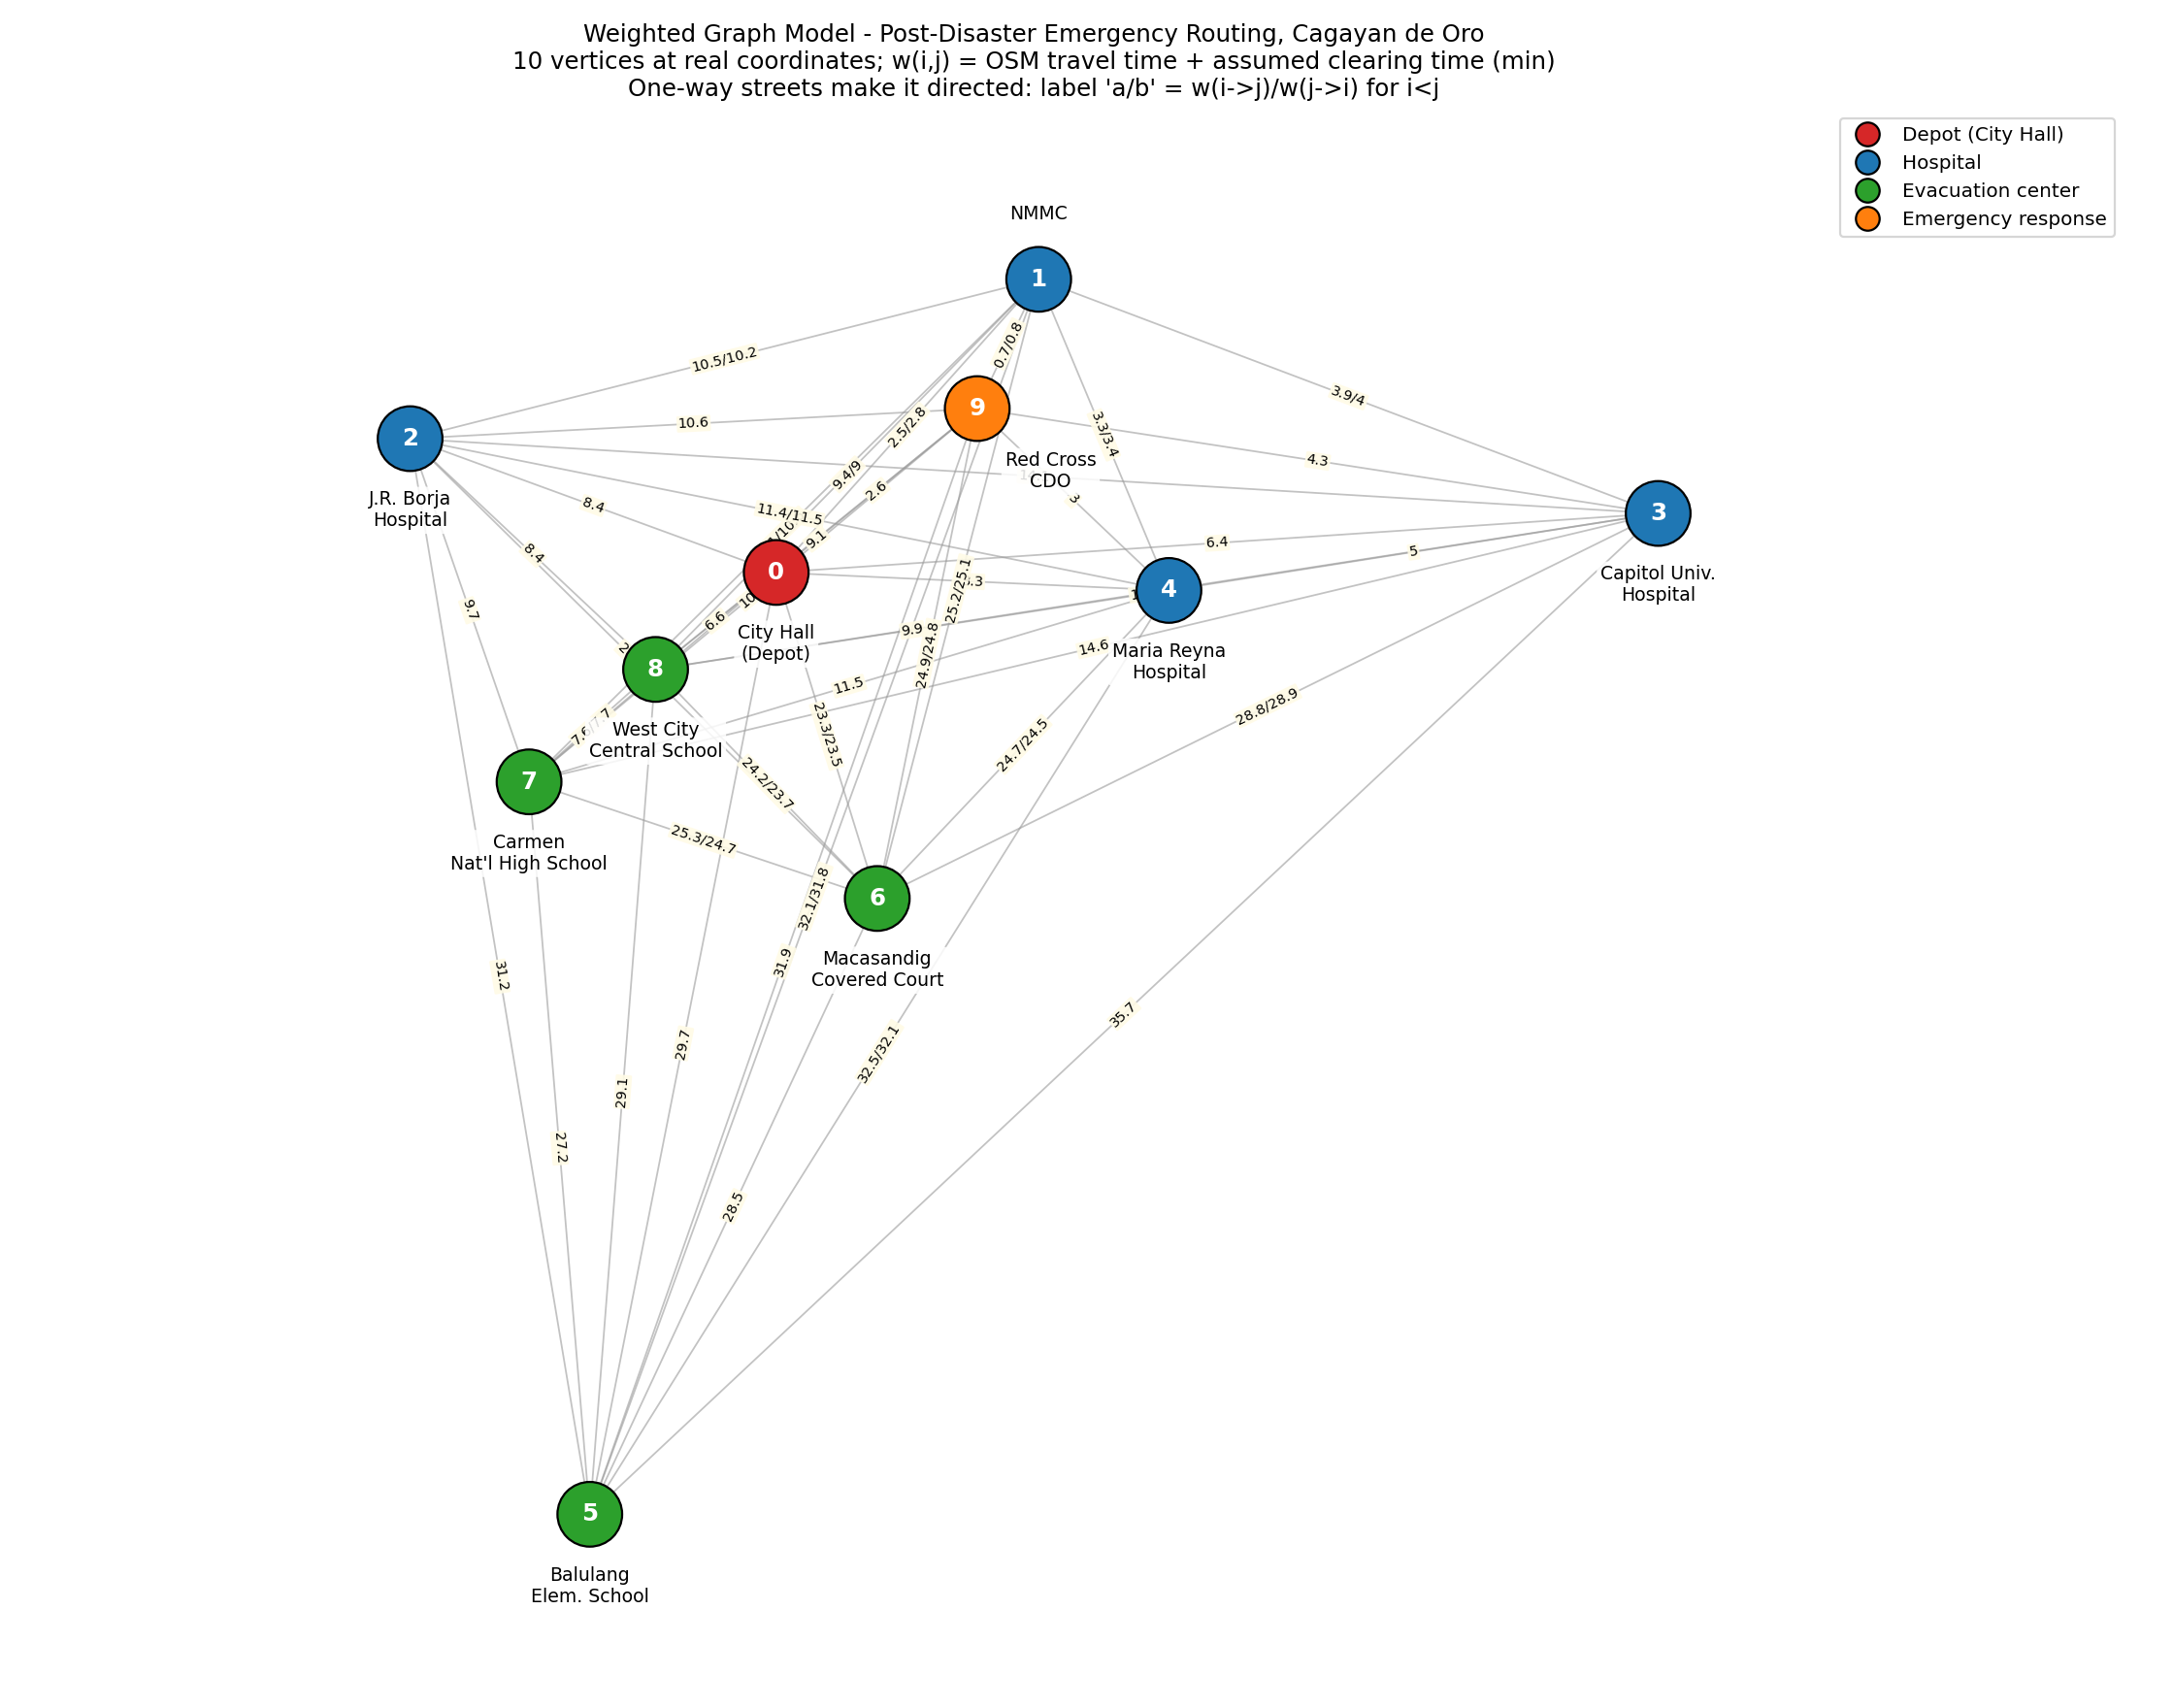
\includegraphics[width=\textwidth]{1_weighted_graph.png}
  \caption{Weighted graph model. Vertex colors give the category; an edge label \emph{a/b} means $w(i\to j)/w(j\to i)$ for $i<j$, and a single number means both directions are equal.}
  \label{fig:graph}
\end{figure}

\subsection{Data pipeline}
The script \texttt{build\_osm\_dataset.py} builds the actual travel-time data in five steps.
\begin{enumerate}[noitemsep]
  \item \textbf{Geocoding.} Each site was located with the OpenStreetMap Nominatim geocoder, and with Overpass API searches for specific buildings where the geocoder returned only a barangay center.
  \item \textbf{Road network.} OSMnx \cite{boeing2017} downloads the drivable network inside the sites' bounding box plus a 0.02$^\circ$ (about 2.2 km) margin. Only the largest strongly connected component is kept, so every site can reach every other. The result has 5,835 intersections and 14,346 directed road segments, and is saved as \texttt{data/cdo\_drive.graphml}.
  \item \textbf{Edge travel times.} Each road segment's speed comes from its \texttt{maxspeed} tag if present, otherwise from Table~\ref{tab:speeds}; its travel time is length divided by speed.
  \item \textbf{Snapping.} Each site is attached to its nearest road intersection by great-circle (haversine) distance; all snaps are within 127 m (Table~\ref{tab:sites}).
  \item \textbf{Shortest paths.} Dijkstra's algorithm \cite{dijkstra1959}, run once from each site, gives the fastest driving time to every other site. Times are rounded to 0.1 minute. The road length along each fastest path is also recorded (Table~\ref{tab:distance}).
\end{enumerate}

\begin{table}[H]\centering\small
\caption{Assumed urban driving speeds by OpenStreetMap road class (km/h); other classes use 20 km/h.}\label{tab:speeds}
\begin{tabular}{lr@{\hspace{2.5em}}lr@{\hspace{2.5em}}lr}
\toprule
Road class & km/h & Road class & km/h & Road class & km/h \\
\midrule
motorway & 60 & primary & 35 & tertiary & 25 \\
motorway\_link & 40 & primary\_link & 25 & tertiary\_link & 20 \\
trunk & 40 & secondary & 30 & unclassified, residential & 20 \\
trunk\_link & 30 & secondary\_link & 25 & service / living\_street & 15 / 10 \\
\bottomrule
\end{tabular}
\end{table}

\subsection{Clearing-time model}
Each site $i$ has an assumed damage class $d_i \in \{0, 5, 20\}$ minutes (Table~\ref{tab:sites}). Reaching or leaving a damaged site requires clearing its access roads, so an edge costs the worse of its two endpoints:
\begin{equation}
  c(i,j) = \max(d_i, d_j), \qquad c(i,i) = 0.
\end{equation}

\subsection{Weight matrices}
Tables~\ref{tab:travel}--\ref{tab:weights} give the three matrices, and Figure~\ref{fig:matrices} shows them as heat maps. Rows and columns 5 and 6 (Balulang and Macasandig) stand out because of their 20-minute clearing penalty.

\TravelMatrix
\ClearingMatrix
\WeightMatrix

\begin{figure}[H]
  \centering
  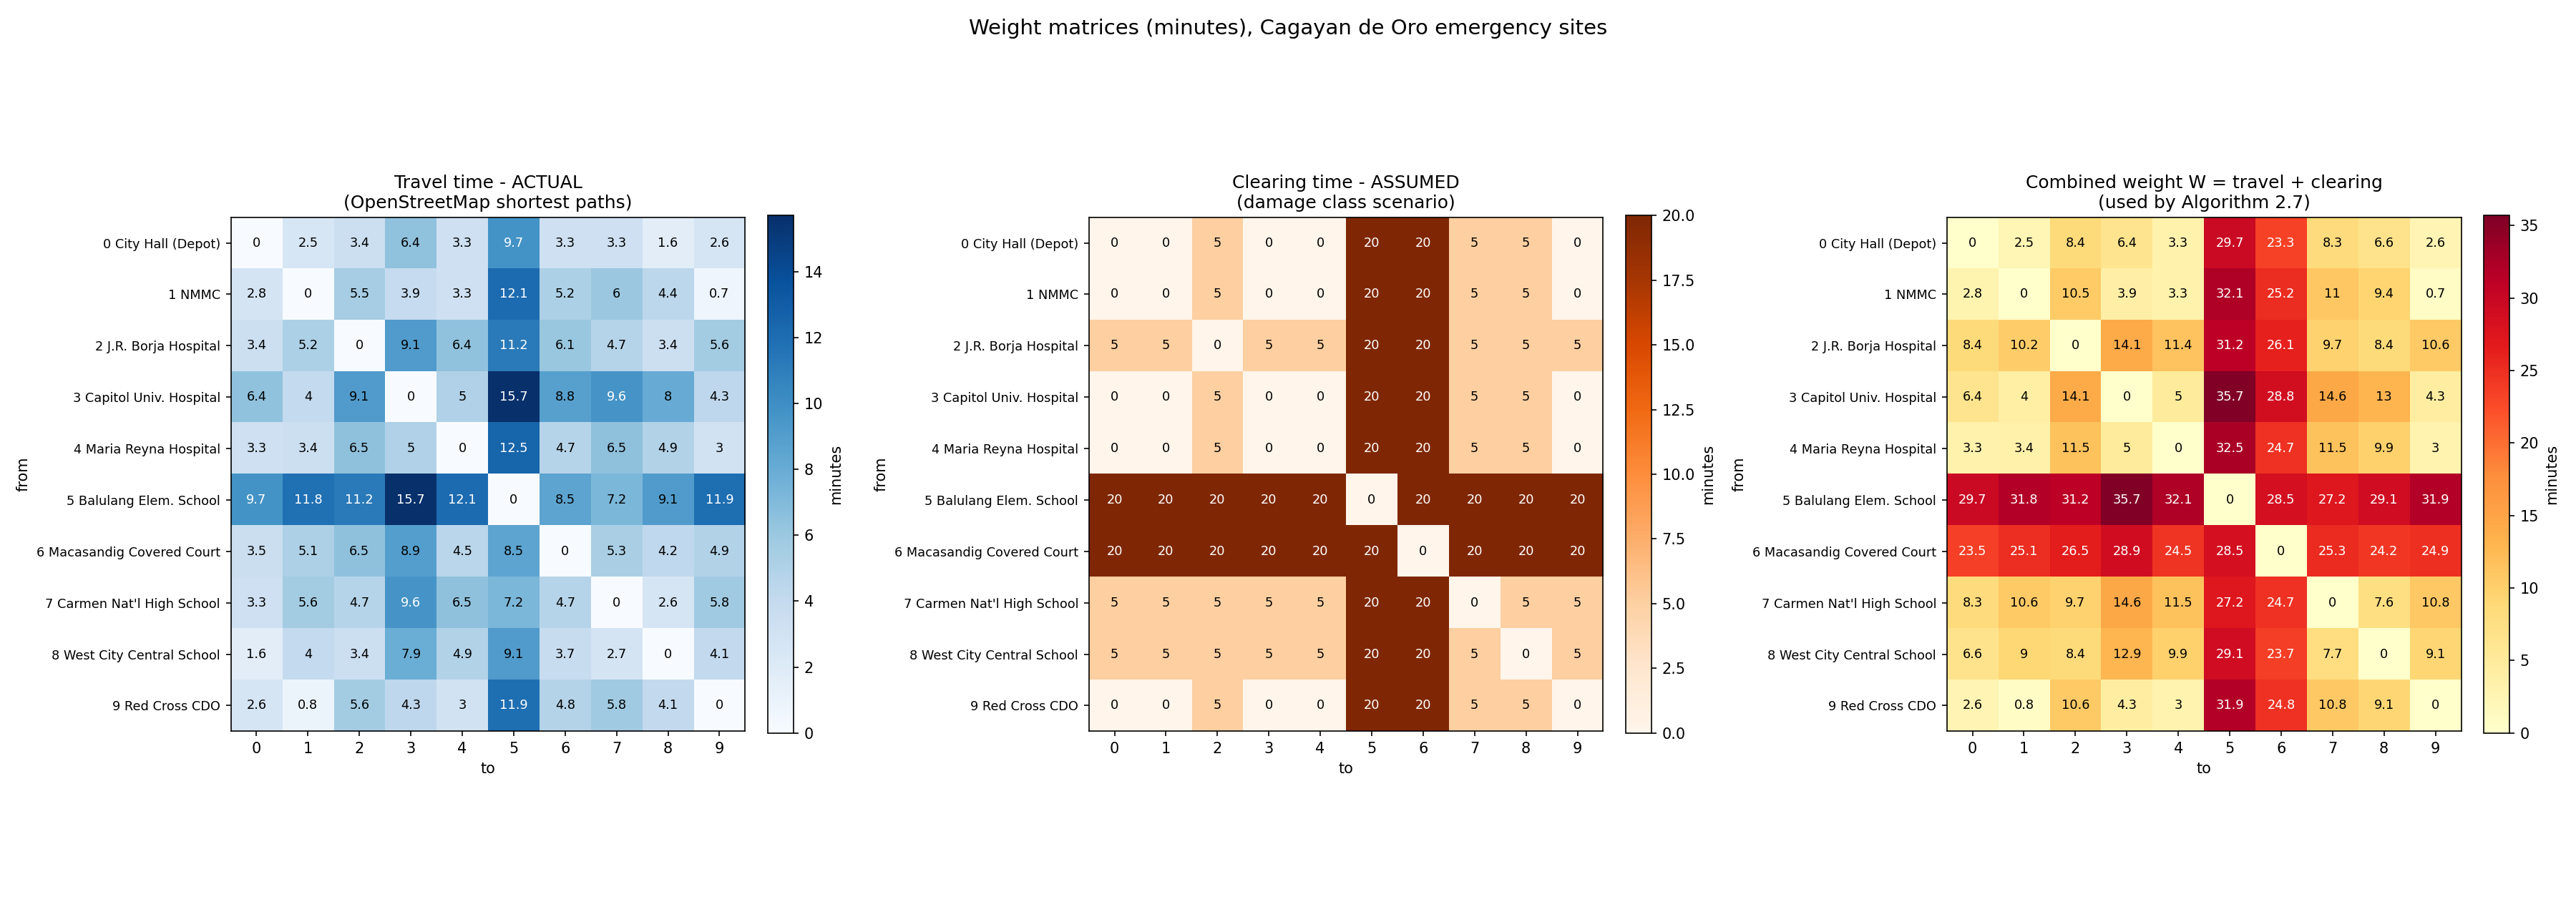
\includegraphics[width=\textwidth]{3_weight_matrices.png}
  \caption{Travel time (actual), clearing time (assumed) and the combined weight matrix used by the algorithm.}
  \label{fig:matrices}
\end{figure}

\subsection{Actual versus assumed data}
\begin{table}[H]\centering\small
\caption{Data sources.}\label{tab:sources}
\begin{tabularx}{\textwidth}{lXl}
\toprule
Data & Source & Type \\
\midrule
Site coordinates & OpenStreetMap via Nominatim and the Overpass API & Actual \\
Road network and road lengths & OpenStreetMap via OSMnx (5,835 intersections) & Actual \\
Route between sites & Dijkstra fastest path on the network & Actual \\
Driving speeds & Road-class speeds, Table~\ref{tab:speeds} & Assumed \\
Clearing times & Damage classes 0 / 5 / 20 min, $c(i,j)=\max(d_i,d_j)$ & Assumed \\
Use of schools as evacuation centers & Scenario choice & Assumed \\
\bottomrule
\end{tabularx}
\end{table}
\noindent OpenStreetMap data was accessed on 17 October 2026. Map data \textcopyright{} OpenStreetMap contributors, available under the Open Database License \cite{osm}.

%=====================================================================
\section{Applying Algorithm 2.7}\label{sec:apply}
%=====================================================================
We run Algorithm 2.7 on the weight matrix of Table~\ref{tab:weights} with the depot, vertex 0, as the start. Table~\ref{tab:steps} traces every step.

\StepTable

The key calculations are:
\begin{itemize}[noitemsep]
  \item \textbf{Step 1.} From City Hall the candidates are NMMC (2.5 min), the Red Cross (2.6 min) and Maria Reyna (3.3 min). NMMC wins by only 0.1 minute.
  \item \textbf{Steps 2--4.} The tour stays among the undamaged north-eastern sites: the Red Cross (0.7), only about 80 m from NMMC, then Maria Reyna (3.0) and Capitol University Hospital (5.0), the easternmost site. The running total is 11.2 minutes after four of ten legs.
  \item \textbf{Steps 5--7.} With the north-eastern sites done, the crew drives west to the minor-damage sites: West City Central School (13.0), Carmen National High School (7.7) and J. R. Borja (9.7).
  \item \textbf{Steps 8--10.} Only the two flooded riverside sites remain, and every remaining edge carries a 20-minute clearing penalty: Macasandig (26.1), Balulang (28.5) and the return to City Hall (29.7). \textbf{These three legs cost 84.3 of the 125.9 minutes.} This is the typical greedy pattern: cheap edges first, expensive edges forced at the end.
\end{itemize}
Adding the chosen weights gives
\[
2.5 + 0.7 + 3.0 + 5.0 + 13.0 + 7.7 + 9.7 + 26.1 + 28.5 + 29.7 = \GreedyTotal{} \text{ minutes.}
\]

\begin{figure}[H]
  \centering
  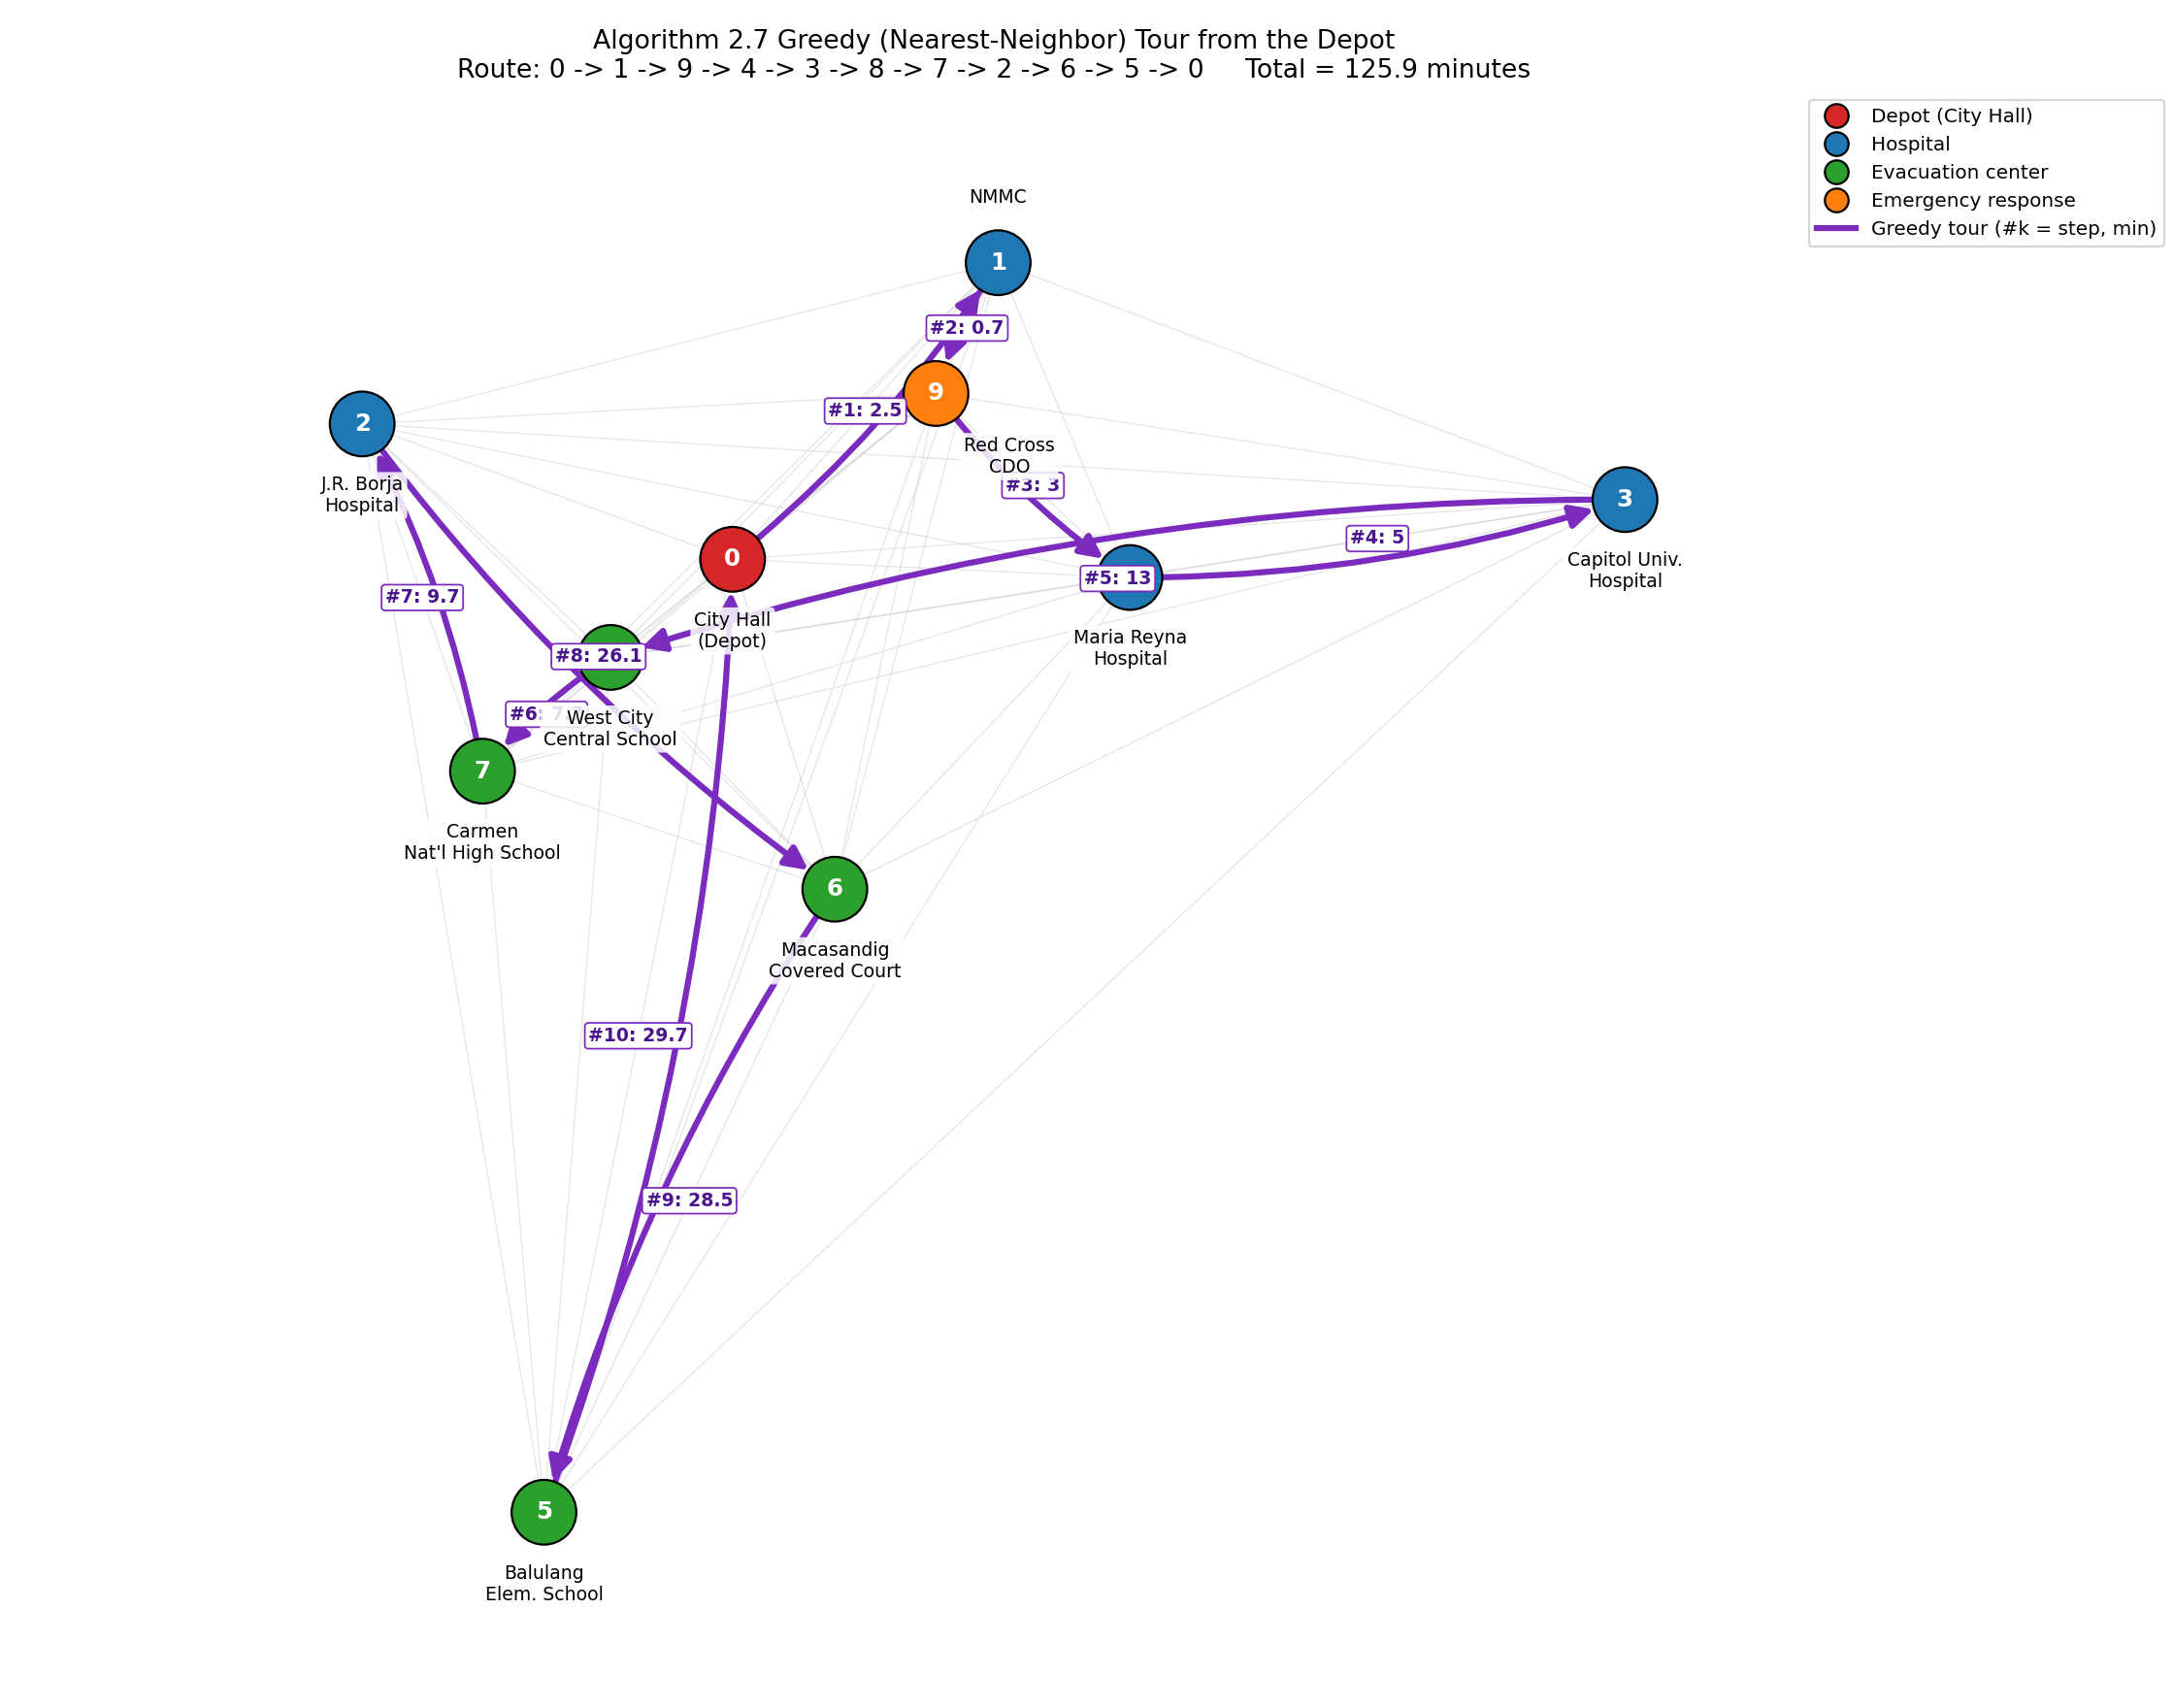
\includegraphics[width=\textwidth]{2_greedy_tour.png}
  \caption{The greedy tour on the graph model. Arrows give the direction of travel; labels \#$k$: $w$ give the step number and the edge weight.}
  \label{fig:greedygraph}
\end{figure}

%=====================================================================
\section{Python implementation}\label{sec:python}
%=====================================================================
\subsection{Structure}
The implementation uses Python 3.13.7 with OSMnx 2.1.1, NetworkX 3.6.1 \cite{hagberg2008} and Matplotlib 3.10.7 \cite{hunter2007}. It consists of three scripts and a \texttt{data/} folder:
\begin{center}\small
\begin{tabularx}{\textwidth}{lX}
\toprule
File & Purpose \\
\midrule
\texttt{build\_osm\_dataset.py} & Downloads the road network, snaps the sites, runs Dijkstra and writes \texttt{data/*.csv} \\
\texttt{tsp\_greedy\_cdo.py} & Site list, weight matrix, Algorithm 2.7, verification and the Held--Karp optimality check \\
\texttt{tsp\_graph\_visualization.py} & Draws the graph, the weight matrices and the route maps in \texttt{figures/} \\
\texttt{data/nodes.csv} & Site coordinates, damage class, snapped OSM node and snap distance \\
\texttt{data/travel\_time\_osm\_min.csv} & $10 \times 10$ travel-time matrix in minutes (the main input) \\
\texttt{data/distance\_osm\_km.csv} & $10 \times 10$ road-distance matrix in kilometres \\
\bottomrule
\end{tabularx}
\end{center}
The scripts are run in this order:
\begin{lstlisting}[style=out]
pip install osmnx networkx matplotlib
python build_osm_dataset.py
python tsp_greedy_cdo.py
python tsp_graph_visualization.py
\end{lstlisting}
The data is not embedded in the code: \texttt{tsp\_greedy\_cdo.py} reads the actual travel times from \texttt{data/travel\_time\_osm\_min.csv}, and the assumed damage classes are in the \texttt{SITES} list at the top of that file. The complete source code is in Appendix~\ref{app:code}.

\subsection{Main components}
\paragraph{Input data.} The \texttt{SITES} list holds each site's name, category, coordinates and assumed damage class. \texttt{load\_travel\_time()} reads the travel-time CSV, \texttt{clearing\_time()} applies $c(i,j)=\max(d_i,d_j)$, and \texttt{load\_weights()} adds them into $W$.

\lstinputlisting[style=py, firstline=66, lastline=76, firstnumber=66, caption={Building the weight matrix (\texttt{tsp\_greedy\_cdo.py}).}]{../tsp_greedy_cdo.py}

\paragraph{Algorithm 2.7.} The function \texttt{greedy\_tsp} follows Algorithm~\ref{alg:formal} line by line. The inner \texttt{for} loop is the ``find the nearest unvisited city'' step; the lines after the \texttt{while} loop close the tour.

\lstinputlisting[style=py, firstline=90, lastline=114, firstnumber=90, caption={Algorithm 2.7 (\texttt{greedy\_tsp} in \texttt{tsp\_greedy\_cdo.py}).}]{../tsp_greedy_cdo.py}

\paragraph{Verification.} \texttt{recalculate} independently sums the edge weights along the returned tour, and the report checks that the visited sites are exactly $\{0,\dots,9\}$ and that the tour returns to the start.

\paragraph{Optimality check.} \texttt{held\_karp} computes the exact optimum by dynamic programming over subsets in $O(n^2 2^n)$ time \cite{heldkarp1962}, which is Algorithm 2.2 of the paper. It is not part of Algorithm 2.7; it is used only to measure how far the greedy result is from the best possible tour.

\subsection{Program output}
The output below is the actual run of \texttt{python tsp\_greedy\_cdo.py} on the dataset in this report.
\lstinputlisting[style=out]{program_output.txt}

%=====================================================================
\section{Results}\label{sec:results}
%=====================================================================
\subsection{Greedy route}
The greedy round trip from City Hall is
\[
0 \to 1 \to 9 \to 4 \to 3 \to 8 \to 7 \to 2 \to 6 \to 5 \to 0,
\]
that is City Hall $\to$ NMMC $\to$ Red Cross $\to$ Maria Reyna $\to$ Capitol University Hospital $\to$ West City Central School $\to$ Carmen National High School $\to$ J. R. Borja $\to$ Macasandig $\to$ Balulang $\to$ City Hall. Its total is \textbf{\GreedyTotal{} minutes}: \GreedyTravel{} minutes of driving and \GreedyClear{} minutes of road clearing, over \GreedyKm{} km of road. Figure~\ref{fig:map} shows the route on the real streets.

\begin{figure}[H]
  \centering
  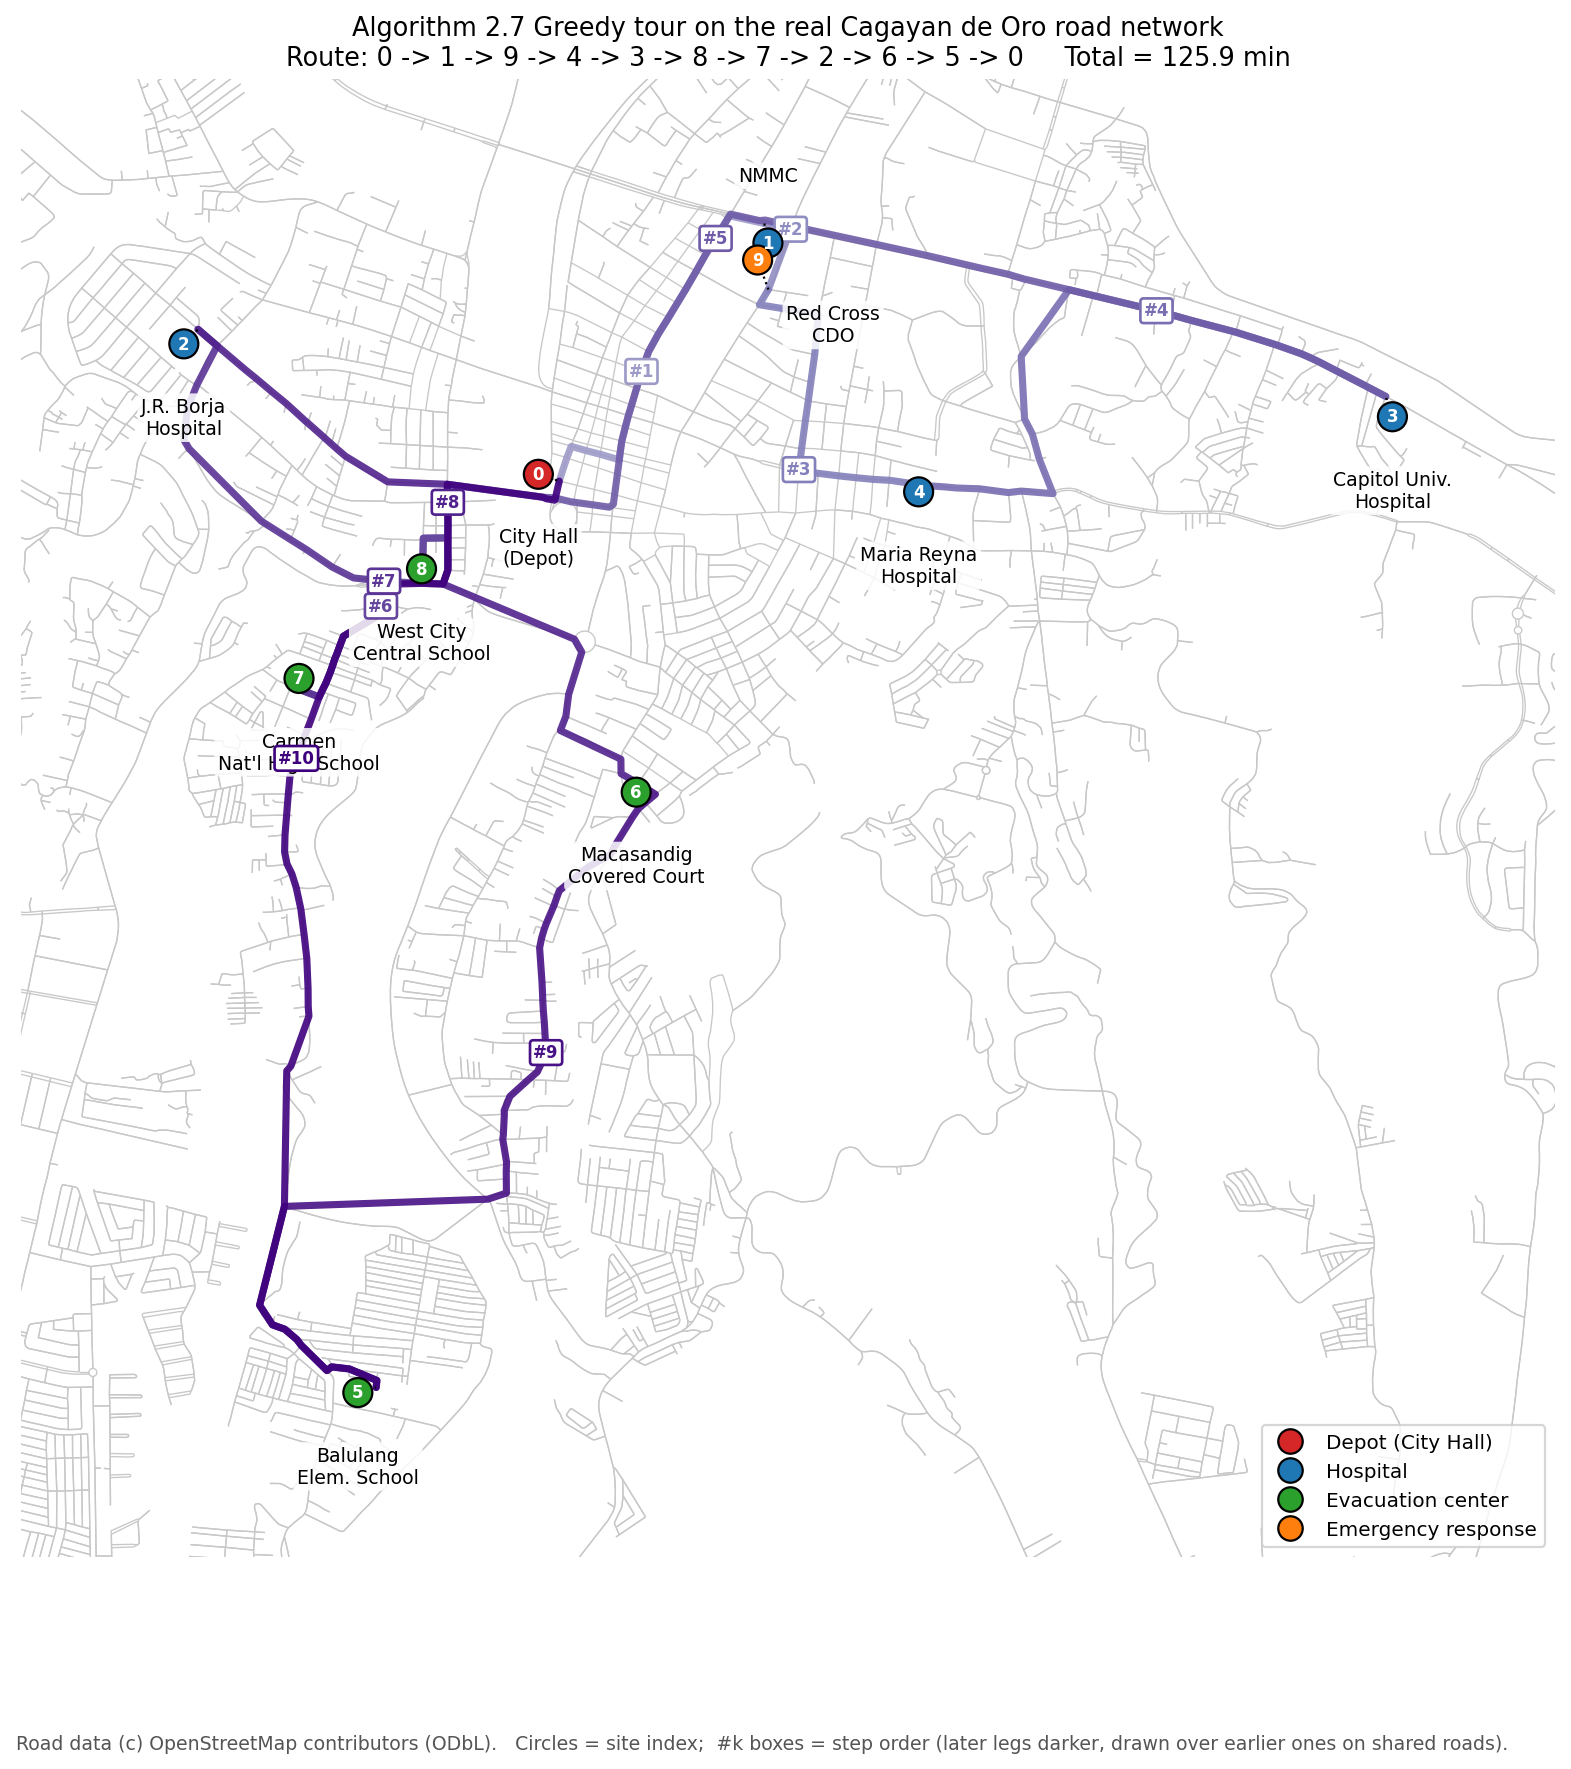
\includegraphics[width=0.78\textwidth]{4_greedy_route_map.png}
  \caption{The greedy tour on the OpenStreetMap road network of Cagayan de Oro. Circles are sites; \#$k$ boxes give the step order. Road data \textcopyright{} OpenStreetMap contributors (ODbL).}
  \label{fig:map}
\end{figure}

\subsection{Verification}
The program output confirms that:
\begin{itemize}[noitemsep]
  \item every one of the ten sites appears exactly once before the return;
  \item the tour starts and ends at City Hall; and
  \item the total recomputed from the edge weights equals the reported total, \GreedyTotal{} minutes. The hand calculation in Section~\ref{sec:apply} gives the same value.
\end{itemize}

\subsection{Comparison with the optimum}\label{sec:optimal}
Because $n = 10$ is small, the exact optimum can be computed. The Held--Karp dynamic program gives the tour in Table~\ref{tab:optimal} with a total of \textbf{\OptTotal{} minutes}. A brute-force search over all $9! = 362{,}880$ tours that start and end at City Hall gives the same tour and total, which confirms that it is optimal for this graph.

\OptimalTable

\begin{table}[H]\centering\small
\caption{Greedy versus optimal tour.}\label{tab:compare}
\begin{tabular}{lrrrr}
\toprule
Tour & Total (min) & Driving (min) & Clearing (min) & Distance (km) \\
\midrule
Greedy (Algorithm 2.7) & \GreedyTotal & \GreedyTravel & \GreedyClear & \GreedyKm \\
Optimal (Held--Karp) & \OptTotal & \OptTravel & \OptClear & \OptKm \\
\bottomrule
\end{tabular}
\end{table}

The greedy tour is \GapMin{} minutes, or \textbf{\GapPct\%}, longer than the optimum. Both tours visit Balulang and Macasandig back to back, so each pays the 20-minute clearing penalty on exactly three edges and both spend the same \GreedyClear{} minutes clearing roads. (A tour that separated those two sites would pay the penalty on four edges.) The whole gap therefore comes from driving, \GreedyTravel{} versus \OptTravel{} minutes: the optimal tour visits the riverside sites in the middle of the trip, while greedy postpones them and then has to drive back to City Hall from Balulang, the farthest site, at the end.

\begin{figure}[H]
  \centering
  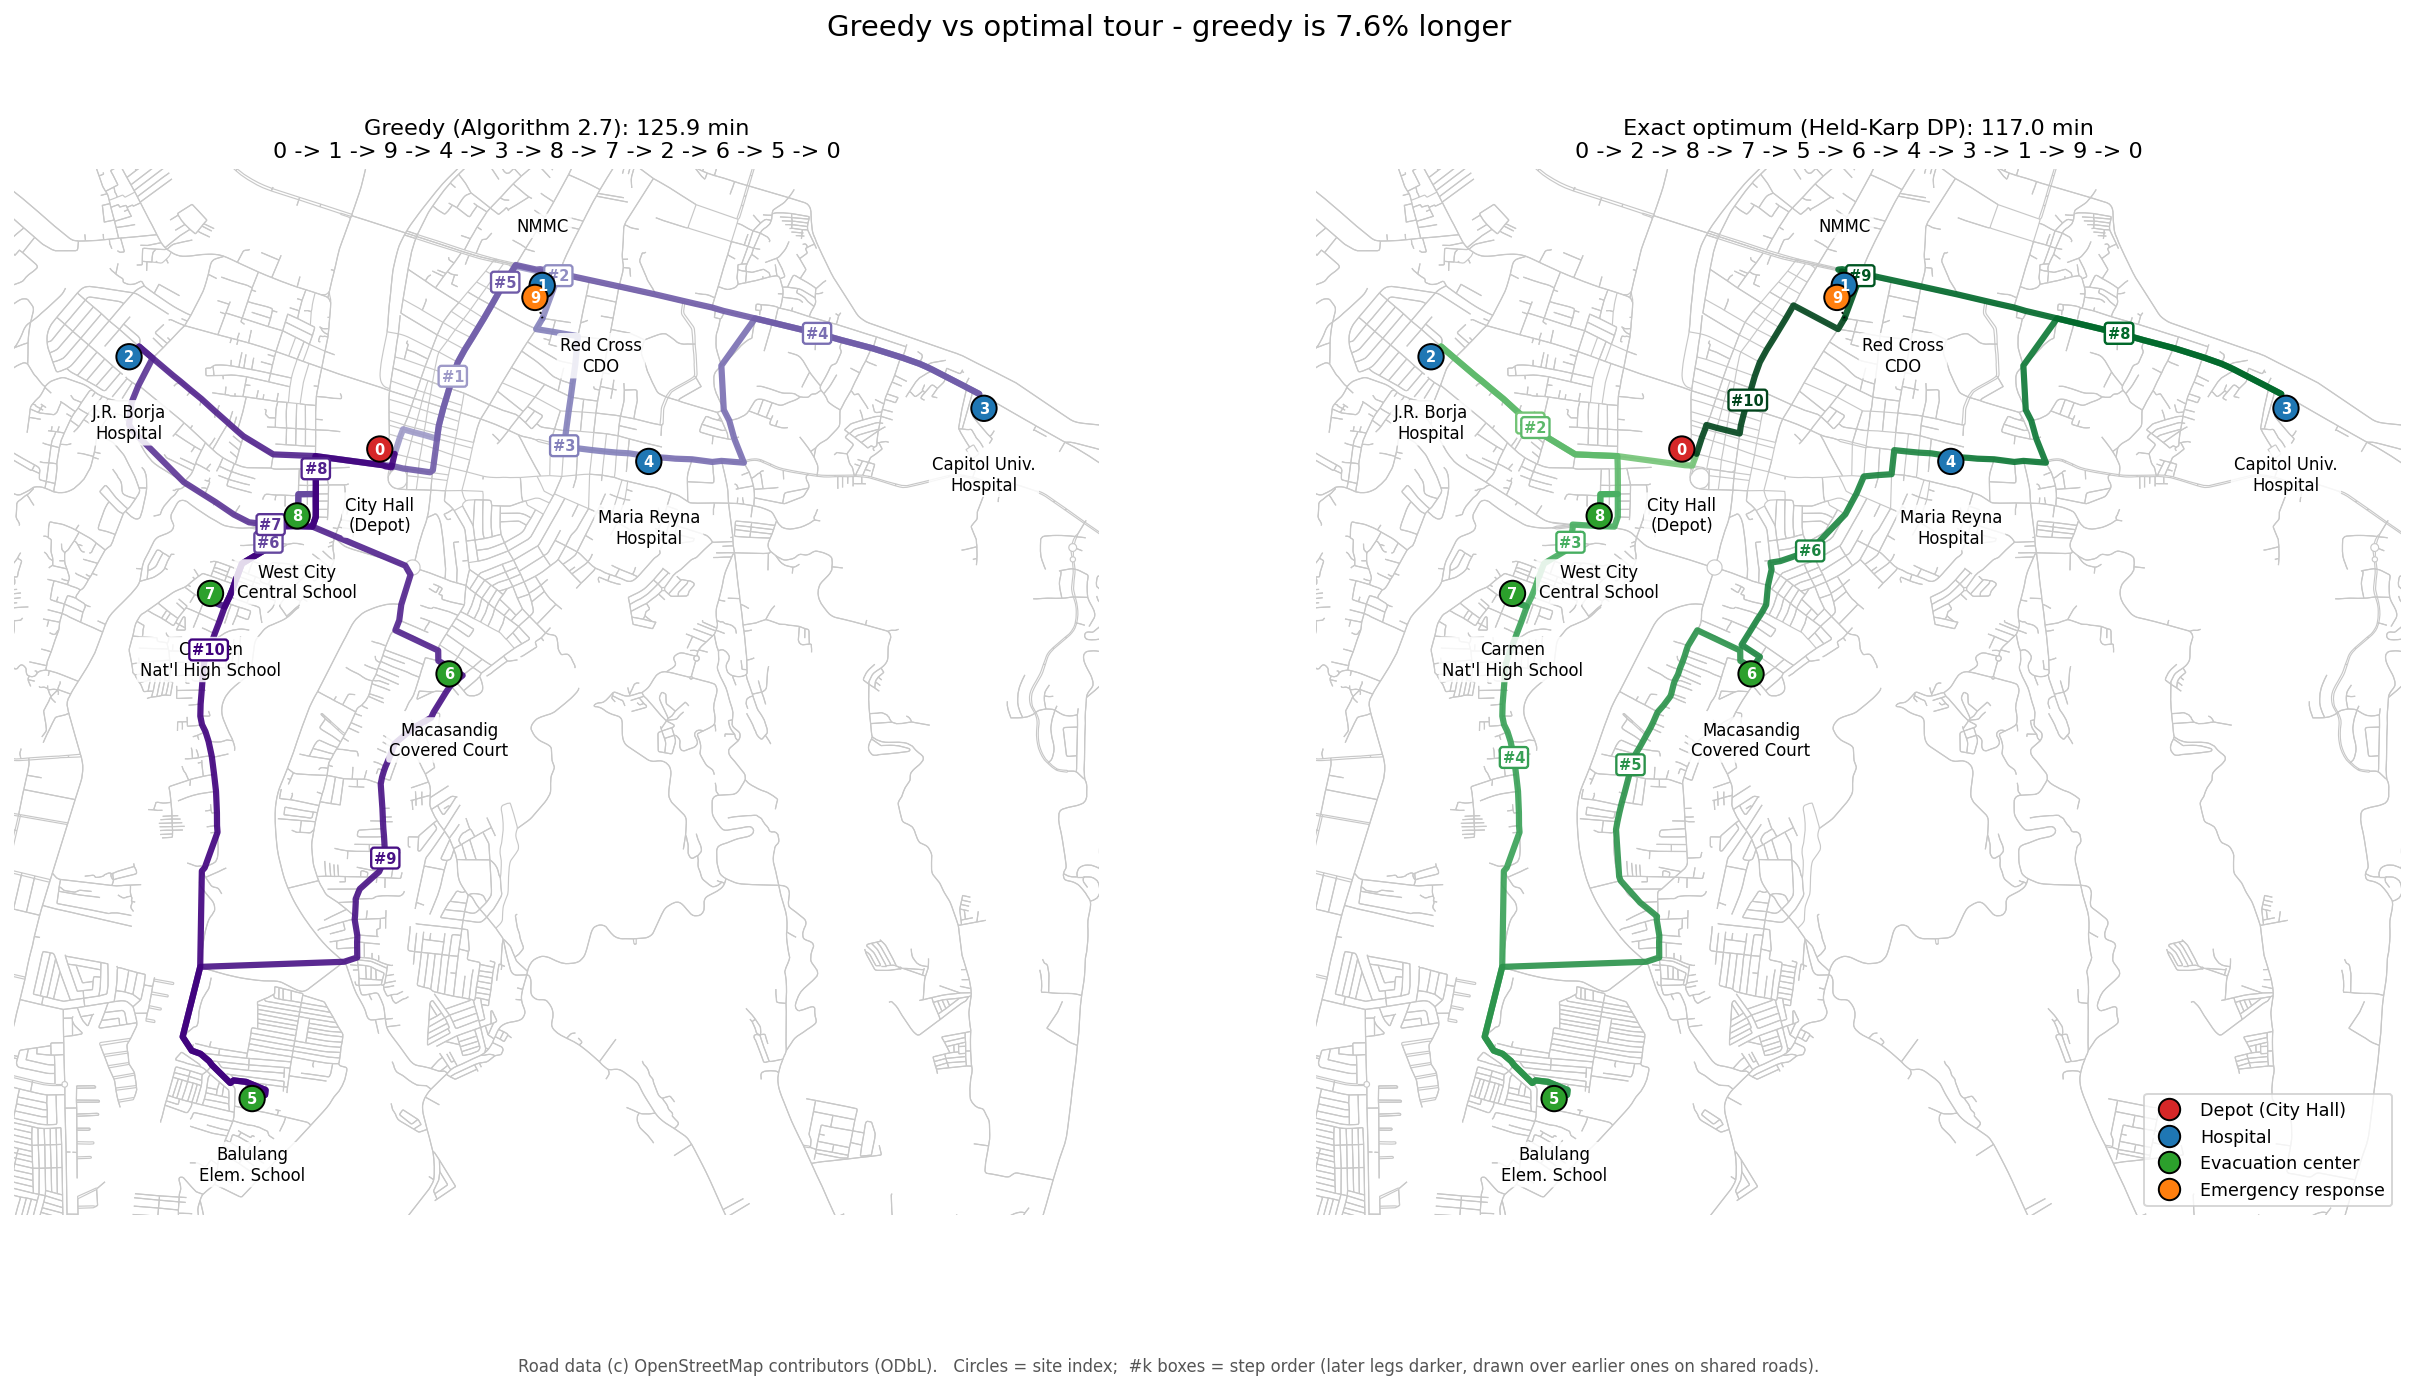
\includegraphics[width=\textwidth]{5_greedy_vs_optimal_map.png}
  \caption{Greedy tour (left, \GreedyTotal{} min) and optimal tour (right, \OptTotal{} min) on the same road network.}
  \label{fig:compare}
\end{figure}

\subsection{Sensitivity to the starting vertex}
Running the greedy algorithm from each of the ten sites gives totals between 121.3 and 130.1 minutes (Table~\ref{tab:sensitivity}). None reaches the optimum of \OptTotal{} minutes, and starting from City Hall is not the best choice. This confirms two of the limitations in Section~\ref{sec:algorithm}: the result depends on the start, and it is not guaranteed to be optimal.

\SensitivityTable

%=====================================================================
\section{Conclusion}\label{sec:conclusion}
%=====================================================================
\subsection{Interpretation}
The greedy route meets the objective of the problem in a practical sense: it gives the emergency crew a valid order in which to reach all four hospitals, four evacuation sites and the response hub, each exactly once, and return to City Hall in \GreedyTotal{} minutes. It is computed in milliseconds and is easy to explain and follow. It is \emph{not} the shortest possible route: the proven optimum is \OptTotal{} minutes, \GapPct\% faster. We claim optimality only for the Held--Karp result, which is supported by both dynamic programming and brute force; the greedy route is an approximate solution.

\subsection{Limitations}
\begin{itemize}[noitemsep]
  \item Driving speeds and clearing times are assumptions, not measurements, so the absolute minutes are estimates.
  \item The road network is static. In a real flood some roads would be closed, and travel times would change during the trip.
  \item The model has no site priorities or time windows, although hospitals may need to be reached first.
  \item Service time at each site and the walk from the road to each building are ignored.
  \item The greedy rule postpones the far, flooded sites to the end of the trip, which is exactly where the gap to the optimum comes from.
\end{itemize}

\subsection{Possible improvements}
\begin{itemize}[noitemsep]
  \item Apply 2-opt local search \cite{croes1958} to the greedy tour to remove its long late legs.
  \item Run the greedy algorithm from every starting vertex and keep the best tour (at $O(n^3)$ cost).
  \item Use live road-closure and traffic data instead of assumed speeds and clearing times.
  \item Add site priorities or time windows to the objective.
  \item Compare with the metaheuristics in the paper: simulated annealing, genetic algorithms and particle swarm optimization \cite{luna2024}.
\end{itemize}

%=====================================================================
\begin{thebibliography}{99}
%=====================================================================
\bibitem{luna2024} R. Luna-Garcia, T. M. C. Candano, and R. L. Caga-anan, ``Performance analysis of classical algorithms for the traveling salesman problem,'' \emph{The Mindanawan Journal of Mathematics}, vol.~6, no.~2, pp.~79--111, 2024. \url{https://doi.org/10.62071/tmjm.v6i2.716}
\bibitem{osm} OpenStreetMap contributors, ``OpenStreetMap data for Cagayan de Oro City,'' Open Database License (ODbL), accessed 17 October 2026. \url{https://www.openstreetmap.org}
\bibitem{boeing2017} G. Boeing, ``OSMnx: New methods for acquiring, constructing, analyzing, and visualizing complex street networks,'' \emph{Computers, Environment and Urban Systems}, vol.~65, pp.~126--139, 2017.
\bibitem{dijkstra1959} E. W. Dijkstra, ``A note on two problems in connexion with graphs,'' \emph{Numerische Mathematik}, vol.~1, pp.~269--271, 1959.
\bibitem{heldkarp1962} M. Held and R. M. Karp, ``A dynamic programming approach to sequencing problems,'' \emph{Journal of the Society for Industrial and Applied Mathematics}, vol.~10, no.~1, pp.~196--210, 1962.
\bibitem{rosenkrantz1977} D. J. Rosenkrantz, R. E. Stearns, and P. M. Lewis, ``An analysis of several heuristics for the traveling salesman problem,'' \emph{SIAM Journal on Computing}, vol.~6, no.~3, pp.~563--581, 1977.
\bibitem{croes1958} G. A. Croes, ``A method for solving traveling-salesman problems,'' \emph{Operations Research}, vol.~6, no.~6, pp.~791--812, 1958.
\bibitem{hagberg2008} A. A. Hagberg, D. A. Schult, and P. J. Swart, ``Exploring network structure, dynamics, and function using NetworkX,'' in \emph{Proceedings of the 7th Python in Science Conference}, pp.~11--15, 2008.
\bibitem{hunter2007} J. D. Hunter, ``Matplotlib: A 2D graphics environment,'' \emph{Computing in Science \& Engineering}, vol.~9, no.~3, pp.~90--95, 2007.
\end{thebibliography}

%=====================================================================
\appendix
\section{Source code}\label{app:code}
%=====================================================================
\subsection{\texttt{tsp\_greedy\_cdo.py}}
\lstinputlisting[style=py]{../tsp_greedy_cdo.py}
\subsection{\texttt{build\_osm\_dataset.py}}
\lstinputlisting[style=py]{../build_osm_dataset.py}
\subsection{\texttt{tsp\_graph\_visualization.py}}
\lstinputlisting[style=py]{../tsp_graph_visualization.py}

\section{Road distances}
\DistanceMatrix

\end{document}
